\documentclass{article} % For LaTeX2e
\usepackage{nips13submit_e,times}
\usepackage{hyperref}
\usepackage{url}
\usepackage{graphicx}
%\documentstyle[nips13submit_09,times,art10]{article} % For LaTeX 2.09


\title{OCR using Machine Learning Techniques and Hidden Markov Models}


\author{
Jonathan Yee\\
\texttt{jyee1@andrew.cmu.edu} \\
\And
Lingzhang Jiang \\
\texttt{lingzhaj@andrew.cmu.edu} \\
}

% The \author macro works with any number of authors. There are two commands
% used to separate the names and addresses of multiple authors: \And and \AND.
%
% Using \And between authors leaves it to \LaTeX{} to determine where to break
% the lines. Using \AND forces a linebreak at that point. So, if \LaTeX{}
% puts 3 of 4 authors names on the first line, and the last on the second
% line, try using \AND instead of \And before the third author name.

\newcommand{\fix}{\marginpar{FIX}}
\newcommand{\new}{\marginpar{NEW}}

\nipsfinalcopy % Uncomment for camera-ready version

\begin{document}


\newcommand{\mycount}{\mbox{count}}

\maketitle

\begin{abstract}
Optical Character Recognition (OCR) has been the focus of much ML research. A reliable OCR system has a wide range of uses, from recognizing scanned books to license plate recognition. Since a sequence of characters (e.g. an English word) is not generated randomly, we can model the process of writing after a Hidden Markov Model (HMM). The hidden states are the letters the human is thinking of, and the observed states are what he or she actually writes. This HMM exploits the correlation between neighboring letters in the general OCR case to improve accuracy. We have found that using Maximum Likelihood Estimates (MLE) to learn the parameters, and using the Viterbi algorithm to find the most likely set of hidden states, leads to a recognition rate of 69.7\%. This is higher than the accuracy rate of using Naive Bayes (62.7\%) and Logistic Regression (64.1\%).
\end{abstract}

\section{Background}
We are trying to apply different machine learning techniques to an Optical Character Recognition (OCR) problem, with the objective of obtaining a high level of accuracy comparable on a given data-set comparable to state-of-the-art techniques.

OCR can be analyzed using the noisy channel model, with the source being the human mind, and the channel being the handwriting technique. We want to determine the most likely letter given the handwriting. 

For this project, we intend to design a Hidden Markov Model. The hidden states of the HMM will be the letters the human is thinking of, and the observed output is the actual handwriting represented as a pixel vector. This HMM can be graphically represented as a Bayes net. The goal is to find the sequence of hidden states (i.e. letters) that maximize the joint probability of those characters and the pixel vectors. Various OCR techniques (neural networks, naive bayes, logistic regression) can be applied to determine the probabilities that a pixel vector is a certain letter. We also intend to use the Viterbi algorithm to determine the most likely sequence of letters.

\begin{figure}[h]
\begin{center}
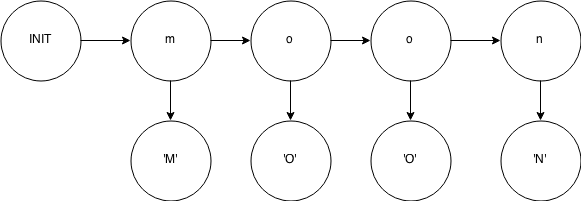
\includegraphics[scale=0.5]{ml_project_hmm.png}
\end{center}
\caption{Hidden markov model for the word "moon". Observed states are the written pixels.}
\label{fig:hmm-letters}
\end{figure}

\section{Related Work}
The first related work we looked at was a similar study by Ivan Dervisevic[1], which utilized four classifiers(Naive Bayes, Complement Naive Bayes, SMO, and C4.5) to perform OCR and compared the results of these classifiers. SMO is a kind of support vector machine classifier while C4.5 is a decision tree classifier. The dataset that was used contained capital characters from 238 TrueType fonts and the data was 40x40 pixel images of each character. In addition to using the raw unprocessed pixel image data, refined datasets with processed representations of the characters were also used. As our focus is more on the machine learning portion and less on the image processing techniques, we will only be using 2 classifiers as a baseline, leaving out image processing, and focusing on implementing a HMM to optimize classification instead.

The second related work we looked at was an introduction to Hidden Markov Models[2] by Rabiner. Since we have not had any comprehensive experience with HMMs, we thought it would be a good idea to see what has already been accomplished with HMMs. In this paper, Rabiner provides a review of the theoretical aspects of using HMMs modeling, and also shows how they apply to machine recognition of speech. This overview serves to provide a good background on the theory and application of HMMs, as well as the limitations that Rabiner discusses in the final section.

\section{Methods}
To obtain our baselines, we picked two machine learning learning methods that were taught in class, Naive Bayes and Logistic Regression. Both of these methods would take as inputs a data array containing the pixel data of a collection of handwritten characters as well as a vector containing the labels for the data array. After training the classifiers on the training set, we ran the trained classifiers on a test data set for which we know the correct labels, and compared the predicted labels with the correct labels to get the accuracy of the classifiers. Also, we did cross-validation to get a confident accuracy rating for our baseline methods. 

As an extension of the baselines, we decided to use MLE to learn the parameters of the HMM. First, we learned the parameters by counting the letters and pixels and calculating the transition and emission probabilities using MLE. Then, we used the Viterbi algorithm to calculate the most likely sequence of hidden states given some test sample. This likely sequence of hidden states corresponds to the recognized letter for each pixel vector. We compared the predicted labels with the correct labels to get the accuracy of the classifiers. Finally, we did cross-validation to get a confident accuracy rating for our extension. 

\section{Experiments}
\subsection{Data Set}
The dataset we are using contains handwritten words. The dataset was collected by Rob Kassel at MIT Spoken Language Systems Group. A subset of the words were chosen and the images of each letter were rasterized and normalized. Since the first letter of each word was capitalized and the rest were lowercase, the first letter was removed and only the lowecase letters were used. The given tab delimited data file  contains a line for each letter, with its label, pixel values, and several additional fields listed in a separate file. 

The data set can be accessed at \url{http://ai.stanford.edu/~btaskar/ocr/}

\section{Results - Baseline}
\subsection{Naive Bayes}
For our first baseline we performed Naive Bayes on the raw pixel data.
If given some character $c$ and an array of n binary pixel values $\{p_1, ..., p_n\}$, the algorithm is based on basic Bayes rule:
$$P(c|p_1, p_2, ... , p_n) = \frac{P(p_1, p_2, ... , p_n|c)p(c)}{p(p_1, p_2, ... , p_n)}$$
If we make the assumptions that individual pixels are conditionally independent given some character then we can expand the conditional probability in the numerator. Using the naive bayes algorithm in the statistics toolbox for Matlab, we ran Naive Bayes over our dataset consisting of pixel data for 52152 characters(26 unique characters, no capitals) with each observation having 128 binary pixel values.

N-fold cross validation splits the data into N disjoint sets. In each of N iterations training is done on N-1 sets and testing is done on the remaining 1 set. If we take the mean accuracy we can then average out errors resulting from variance.


\begin{table}[h]
\centering
\begin{tabular}{|c|c|}
\hline
Iteration & Accuracy \\
\hline
1 & 62.53\% \\
2 & 61.94\% \\
3 & 62.93\% \\
4 & 62.86\% \\
5 & 63.67\% \\
6 & 62.58\% \\
7 & 62.59\% \\
8 & 62.99\% \\
9 & 61.84\% \\
10 & 62.84\% \\
\hline
Avg & 62.7\% \\ 
\hline
\end{tabular}
\caption{Output of training and testing MLE-learned HMM over some number of iterations}
\label{tab:mid-logr-results}
\end{table}

We performed 10-fold cross validation for our Naive Bayes classifier and were able to obtain a final accuracy of 62.7\%.

\subsection{Logistic Regression}
The other classifier that we chose for our baseline is logistic regression.
Logistic regression transforms a given binomial dependent variable, eg. the result of a coin toss, and applies the logistic function to it, effectively transforming it into a continuous variable, as such:
$$F(x) = \frac{1}{1+e^{-(-\beta_0 + \beta_1x)}}$$
The logistic function is useful because it is a function mapping from real numbers to an interval between 0 and 1, and hence the output can be treated as a probability. The logistic regression algorithm itself then follows an approach similar to linear regression to train a set of weight($\beta_0, \beta_1...$) that maximizes the likelihood of the data.

In our case, as we have 26 unique characters which cannot be represented by a binomial variable, we chose to use the multinomial logistic regression algorithm(mnrfit) provided in the statistics toolbox in Matlab. The model takes basically the same principles governing logistic regression for a binary dependent variable, except that it assigns one of the categories for the dependent variable as a 'reference category', and calculates the probabilities of an observation being in each of the other categories as opposed to being in the reference category. For the parameters we used the nominal(default) model, as there is no natural ordering among our response variable categories that would better suit an ordinal model.

When running the logistic regression algorithm, we noticed an abnormally long run time. Hence, we eventually reduced the number of examples in the data to 2000 as well as using principal component analysis to reduce the dimensionality of the data down to 50 features. Even so, there were warnings that the model failed to converge. We suspect that this could be a result of the sparseness of the data matrix as each of the raw pixel values can only take on a value of 0 or 1.

\begin{table}[h]
\centering
\begin{tabular}{|c|c|}
\hline
Iteration & Accuracy \\
\hline
1 & 63.00\% \\
2 & 65.00\% \\
3 & 64.25\% \\
4 & 62.25\% \\
5 & 66.00\% \\
\hline
Avg & 64.1\% \\ 
\hline
\end{tabular}
\caption{Output of training and testing MLE-learned HMM over some number of iterations}
\label{tab:mid-logr-results}
\end{table}

In any case, after 5-fold cross validation, we were able to obtain a mean accuracy of 64.1\% which is still slightly better than Naive Bayes.

\subsection{Baseline Comparison}
When running the classification, we also obtained the confusion matrices, and below is a visualization of the average confusion matrix from Naive Bayes and Logistic Regression respectively.

\begin{figure}[h]
\begin{center}
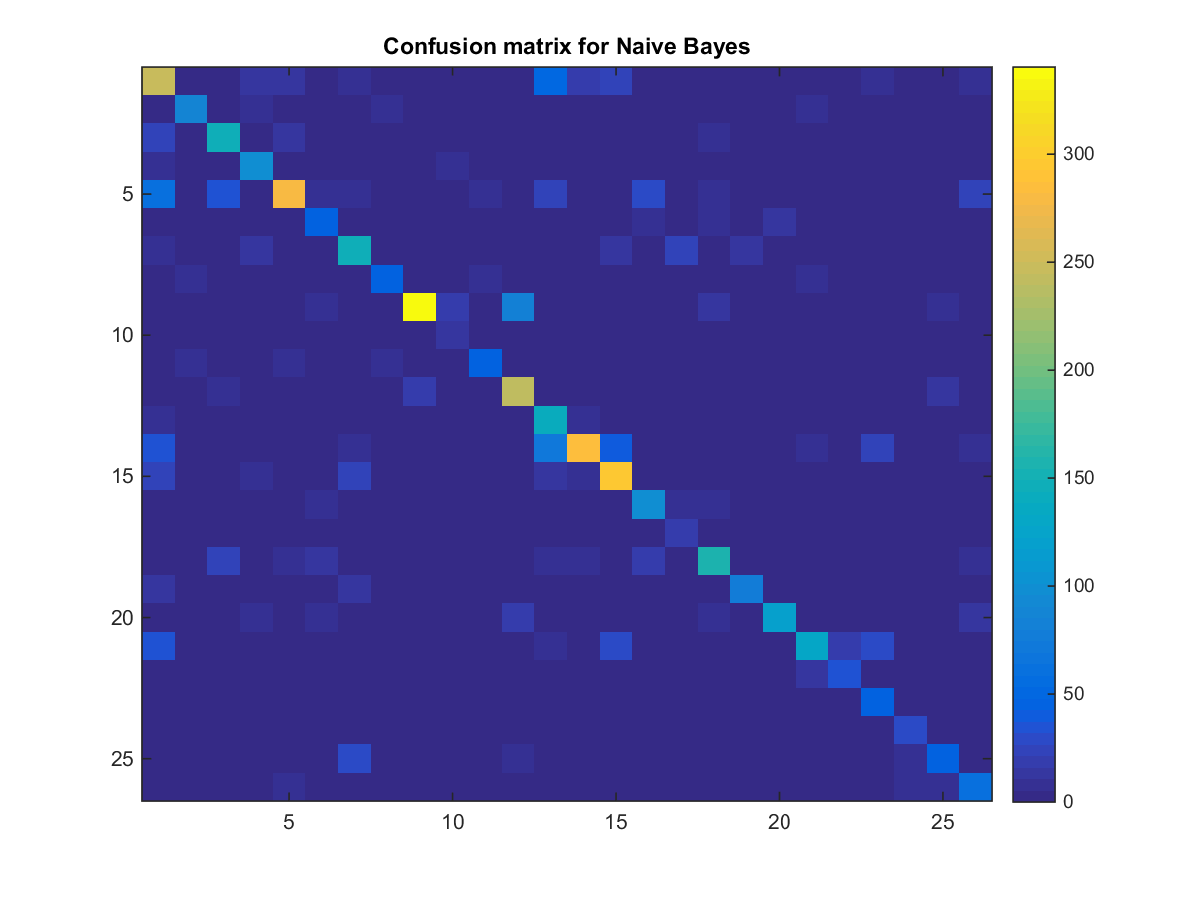
\includegraphics[scale=0.3]{confusionnb.png}
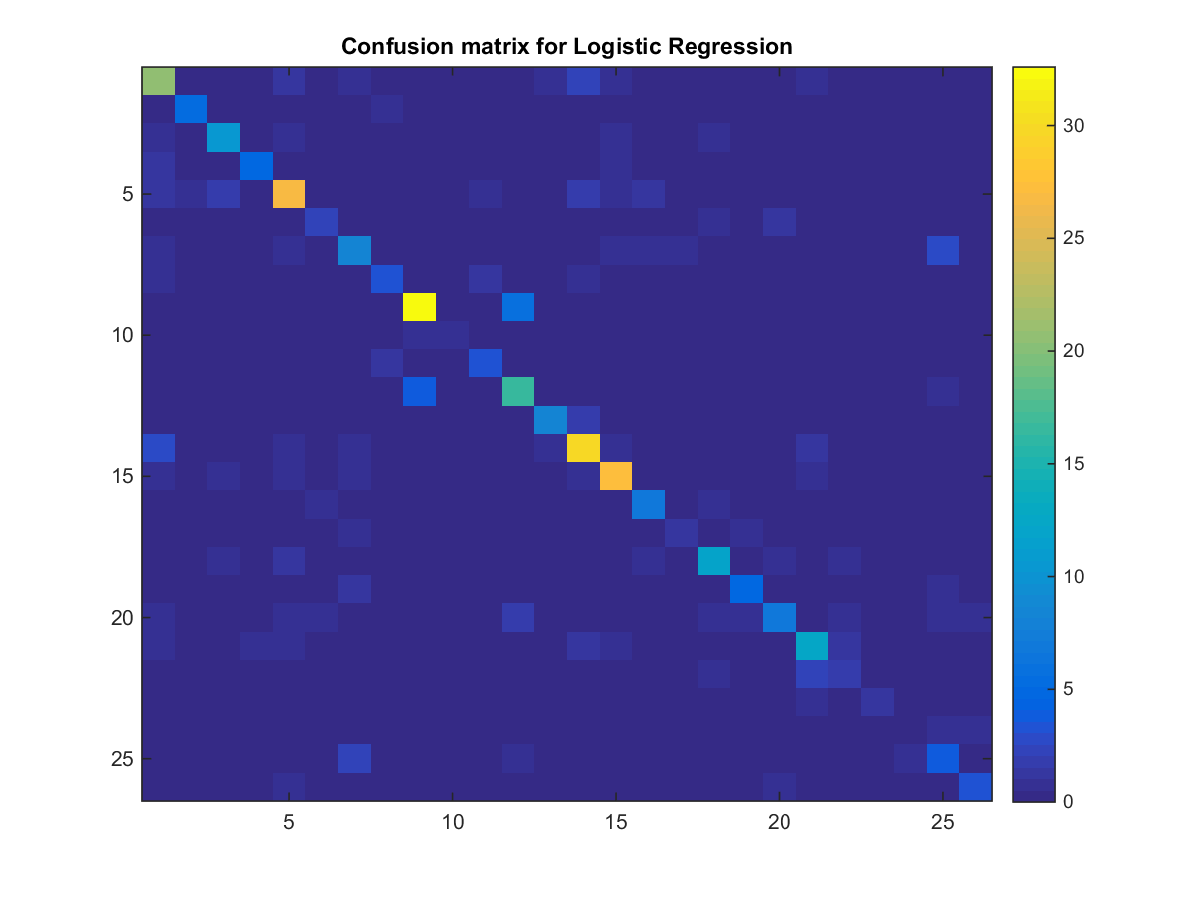
\includegraphics[scale=0.3]{confusionlr.png}
\end{center}
\caption{Visualization of the confusion mats for baseline classifiers}
\end{figure}

A given square $C(i, j)$ shows the number of examples that are known to be in category $i$ but are classified to be in category $j$. A brighter colored square indicates that more examples fall under this description.

We can observe that there are some noticeable patterns for both classifiers just by looking at Figure 1. For example, We see that most of the z's have been classified correctly for both classifiers as the last row is close to being consistently dark blue except at the last square.

Also, for naive bayes, we see that there seems to be a lot of confusion in classifying n(row 14), which seems to be commonly misclassified as n and o, which makes logical sense. 


\section{Results - Intermediate}

\subsection{MLE-Learned HMM Parameters}

We can model a sequence of handwritten letters using a Hidden Markov Model (see Figure~\ref{fig:hmm-letters}). Each hidden state is a letter $c$. Each observed state is a pixel vector $v, v_i \in \{0,1\}$, with length 128 (this is a $16 \times 8$ image). 

To obtain a Hidden Markov Model, we need to find the following parameters:
\begin{itemize}
	\item $\pi_i$ : transition probability from state \texttt{INIT} to $i$
	\item $\phi_{i,j}$ : transition probability from state $i$ to $j$
	\item $\theta_{i}(v)$ : emission probability associated with state $i$ of a pixel vector $v$
\end{itemize}

We plan to use Maximum Likelihood Estimates to find $\phi_{i,j}$. Let $c_1, c_2$ be consecutive letters. Then this is equivalent to finding $P(c_2 | c_1)$. This can be calculated using MLE as follows:
$$ P(c_2 | c_1) = \frac{\mycount(c_1, c_2)}{\mycount(c_1)}$$
We are counting the number of times the bigram $<c_1, c_2>$ appears, and dividing by the number of times $<c_1>$ appears.

To find $\theta_{i}(v)$, we find $P(v | c)$ where $c$ is the letter that is associated with state $i$. Assume Naive Bayes (conditional independence) assumption on $P(v | c)$, so we have 
$$ P(v | c) = \prod_i P(v_i | c)$$
This can be obtained from the training data by looking at all pixel vectors for letter $c$, and applying MLE to calculate $P(v_i = 0 | c)$ and $P(v_i = 1 | c)$ using the frequencies of the pixels that are 0 or 1. In other words,
$$ P(v_i = 1 | c = l) = \frac{\mycount(c = l, v_i = 1)}{\sum_{j=0}^1 \mycount(c = l, v_i = j)}$$

% INSERT VITERBI ALGO HERE

A word is a sequence of letters $Y = <c_1, c_2, ..., c_n>$ with an accompanying sequence of pixel vectors $<v_1, ..., v_n>$, where $n$ is the length of the word. To classify a word, feed the above parameters into the Viterbi algorithm, with the observed states as $v_1, ..., v_n$ to obtain the most likely path of hidden states $\hat{Y} = <c_1, ..., c_n>$, which are the letters. We can then compare the sequence $\hat{Y}$ to the correct labels $Y$ and derive the accuracy of the MLE-learned HMM at OCR.

\begin{table}[h]
\centering
\begin{tabular}{|c|c|}
\hline
Iteration & Accuracy \\
\hline
1 & 69.77\% \\
2 & 70.08\% \\
3 & 67.72\% \\
4 & 70.61\% \\
5 & 70.11\% \\
\hline
Avg & 69.7\% \\ 
\hline
\end{tabular}
\caption{Output of training and testing MLE-learned HMM over some number of iterations}
\label{tab:mle-hmm-results}
\end{table}

% INSERT CONFUSION MATRIX HERE

After 5-fold cross validation, we were able to obtain a mean accuracy of 69.7\% (see Table~\ref{tab:mle-hmm-results}), which is more than 5\% better than either Naive Bayes or Logistic Regression.


\subsection{MLE-Learned HMM Comparison to Baseline}

The mean accuracy of the MLE-learned HMM (69.7\%) is more than 5\% more accurate than either the Naive Bayes classifier (62.7\%) or the Logistic Regression classifier (64.1\%). We theorize that this is because the HMM model accounts for the transitions between letters, hence is more likely to predict a character that, in the training data, has appeared after the previous character.

One of the shortcomings thus far might be the Naive Bayes assumption on the pixel vector, where we assume that the value of each pixel is independent of other surrounding pixels, given the same character. This is unfortunately not true, since a writing instrument is likely to have a line-width of more than 1 pixel. Furthermore, writing often happens in sets of continuous strokes. This implies that if one pixel is switched on, it is more likely that the surrounding pixels are switched on than not.

Another shortcoming is the assumption of the hidden states as being a modeled as per figure ~\ref{fig:hmm-letters}. This assumption lets us use MLE to calculate the transition states. This assumption may result in lower performance, and we will have to wait until we use the Baum-Welch algorithm to estimate the transition and emission probabilities without any assumptions on the hidden states in the learning phase.

\section{Results - Final}

SVM and HMM are da bomb.

\section{Conclusion}

$x$ is clearly better than $y$ and $f$ this class.

\subsubsection*{References}

\small{
[1] Ivan Dervisevic(2006) {\it Machine Learning Methods for Optical Character Recognition.} \url{http://perun.pmf.uns.ac.rs/radovanovic/dmsem/complete/2006/OCR.pdf}

[2] Lawrence R. Rabiner (1989) {\it A Tutorial on Hidden Markov Models and Selected Applications in Speech Recognition} \url{http://www.ece.ucsb.edu/Faculty/Rabiner/ece259/Reprints/tutorial\%20on\%20hmm\%20and\%20applications.pdf}
}

\end{document}
